\section{Bakgrund}

Projektet började våren 2013 som ett internt verktyg på Developer's Helsinki efter ett behov uppstått för ett system som skulle tillåta snabb implementation av anpassat innehåll på kunders webbsidor.

Eftersom det i den tiden inte fanns någon färdig implementation att använda, bestämdes det att det skulle uvecklas en mjukvara först för internt bruk men med målsättningen att lanseras som en SaaS produkt.

\subsection{Developer's Helsinki}

Developer's Helsinki Oy är ett finskt företag som utvecklar såväl applikationestjänster (jmfr. engelskans \gls{saas}) som webbsidor. Företaget grundades 2009 för att vidareutveckla  \gls{saas} tjänsten Netmonitor, en produktfamilj av webbanalys och marknadsföringsverktyg.

Företaget har en stark kännedom av marknadsföring på webben efter att ha jobbat med både utvecklingen av webbsidor samt uppföljningen av resultat genom webbanalys. På basis av denna erfarenhet började SmartElement projektet planeras. Kunskapen fanns inom företaget och genom att anpassa processer från webbanalys sågs en möjlighet för automatisering av anpassning av innehåll.

\subsection{Anpassat innehåll}

\begin{figure}[h!]
\centering
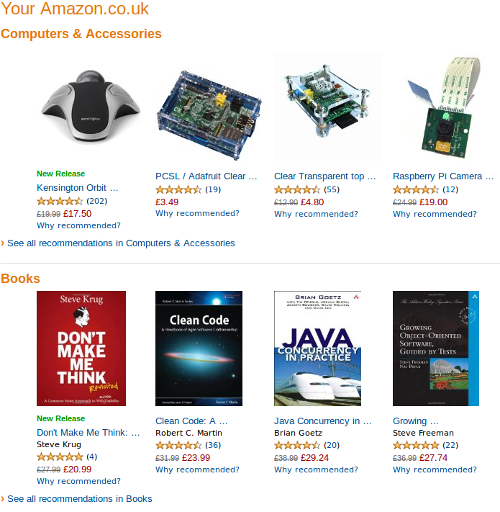
\includegraphics[width=120mm]{assets/images/amazon.png}
\caption{Amazons användarsida med anpassat innehåll}
\label{amazon}
\end{figure}

Anpassat innehåll, eller personaliserat innehåll (eng. \textit{Personalized content}), är innehåll som väljs ut på basis av egenskaper hos användaren. I fallet av webbsidor kan det handla om information som användarens geografiska läge, användarens språk, användarens webbläsare, antalet besök som användaren gjort till sidan m.m. Tanken är att förse användaren med det den behöver, eller vill ha, utan att denne behöver be om det. \citep{cotacm43}

Anpassat innehåll har bland annat användts inom nätbutiker för att visa reklam anpassad för kunden på basis av dennes beställningshistorik. Bild \ref{amazon} visar användarsidan som visas då man loggar in på Amazons webb-butik. Inom social media används anpassat innehåll för att lyfta fram innehåll som antas vara intressant för användaren, som till exempel uppdateringar från vänner som användaren ofta är i kontakt med, reklam från företag användaren har gillat, med mera. \citep{socialmedia}


\subsection{Behov}

I takt med att stora aktörer införde allt mer anpassat innehåll så började även mindre kunder fråga om möjligheten att använda tekniken på sina webbsidor. Det visade sig att det inte fanns något företag på finska marknaden som erbjöd ett tillräckligt flexibelt system för anpassning av innehåll och därmed bestämdes det att Developer's Helsinki skulle utveckla ett sådant.

Systemet skulle kunna leverera innehåll dels i form av text (HTML eller rå text) för direkt injicering i webbsidans \gls{dom}, dels i form av data i \gls{json} format och dels som \gls{jsonp} svar, vilket tillåter exekvering av JavaScript vid svaret. För filtrering skulle det samlas in data om besökares webbläsare och dator, men det skulle även vara möjligt att tillägga egen data som sedan kunde användas för filtrering.

\subsection{Befintliga lösningar}

Vid tillfället för beslutet att utveckla produkten var den enda liknande lösningen på finska marknaden nosto.com som levererar anpassat innehåll med inriktning på webbutiker.\citep{nosto} På grund av produktens klara vinkling\todo{Förklara vinkling} passade den inte in i alla de användningsområden var SmartElement skulle användas.


% vim: set tw=78:ts=2:sw=2:et:fdm=marker:wrap:wm=78:ft=tex
% vim: spell spelllang=sv
